\documentclass[12pt,a4paper]{article}
\usepackage[utf8]{inputenc}
\usepackage{graphicx}
\graphicspath{{../Images/}}
\usepackage{amsmath}
\usepackage{amsfonts}
\usepackage{amssymb}
\usepackage{hyperref}
\usepackage[margin=1in]{geometry}
\usepackage{subfig}
\usepackage{float}
\usepackage{xcolor}

\author{Thibaut Marmey}

\title{Notes de cours R}
\begin{document}
	\maketitle

\begin{normalsize}
\tableofcontents
\end{normalsize}

\section{Programmation R}
\subsection{Généralité}
\begin{itemize}
\item \href{https://openclassrooms.com/fr/courses/1393696-effectuez-vos-etudes-statistiques-avec-r/1394570-les-facteurs#/id/r-1395598}{\textit{lien internet : }reprise cours OCR}
\item \href{https://linuxconfig.org/rstudio-on-ubuntu-18-04-bionic-beaver-linux}{\textit{lien internet : }doc d'installation de R et Rstudio}
\item Utilisation de la documentation "aide" : \textit{help()} ou \textit{help("nom de la fonction")} ou  \textit{?log}
\item Documentation plus détaillée sur internet : \textit{help.start()}
\item Interaction avec l'environnement R :
\begin{itemize}
\item liste toutes les variables crées : \textit{ls()}
\item liste des variables avec une succession de lettre particulière : \textit{ls(pattern="mot")}
\item supprimer des variables : \textit{rm(var)}
\item quitter le travail : \textit{q()} ou \textit{quit()}
\end{itemize}
\item Ecrire des commentaires avec "\#"
\item Utiliser la fonction \textit{print()} pour afficher les informations, textes sur la console
\item Enregistrer les variables que l'on veut : 
\newline \textit{save(var1, var2, ..., file = "nameFile.extension")}.
\newline Enregistrement de ces fichiers dans le répertoires associés \textit{Tools/Global Options}, ici c'est Documents/Notes-de-cours/Cours R/Test
\end{itemize}

\subsection{Fonctions}
\begin{itemize}
\item Tester le type d'une variable :
\begin{itemize}
\item \textit{is.character(var)}
\item \textit{is.numeric(var)}
\item \textit{is.logical(var)}
\item \textit{is.vector(var)}
\item \textit{is.factor(var)}
\item \textit{is.list(var)}
\end{itemize}
\item Spécifier le typage de la variable :
\begin{itemize}
\item \textit{as.numeric(var)}
\item \textit{as.logical(var)}
\item \textit{as.character(var)}
\end{itemize}
\item Renvoyer l'entier inférieur : \textit{floor(nb)}
\item Renvoyer l'entier supérieur : \textit{ceiling(nb)}
\item Arrondir à l'entier le plus proche : \textit{round(nb)}
\item Racine carré : \textit{sqrt()}
\item Fonction trigo : \textit{cos(angleRad), sin, ...}
\item Fonction somme : \textit{sum(vect)}
\item Longueur vecteur : \textit{length(vect)}
\end{itemize}

\subsection{Manipulation de chaînes de caractères}
\begin{itemize}
\item Saisir des données depuis le clavier : \textit{scan()}. Pour valider l'input appuyer sur \textit{entrée}, et un nouvel input appararaîtra. Pour arrêter la prise d'input appuyer directement sur \textit{entrée}.
\item Rentrer le nombre d'input avec l'appel de \textit{scan(nmax=n)}
\item La concaténation de texte et nombre avec \textit{paste(texte, nombres, ...)}
\item Combinaison de \textit{scan()} et \textit{paste()} : \textit{paste('Bonjour j'ai ', scan(nmax=1), ' ans')}
\item Permet de compter le nombre de lettres présentes dans la chaîne de caractères : \textit{nchar("chaîne")}
\item Mettre les caractères en majuscules ou minuscules : \textit{toupper(), tolower()}
\item Extraire une sous chaîne de caractères avec point de départ et d'arrivée inclus : \textit{substr("chaine", start, stop)}. La chaîne de caractères commence à 1.
\end{itemize}

\subsection{Gestion de données complexes}
\begin{itemize}
\item Le vecteur : élément de base du langage, c'est une liste d'éléments étant tous du même type. Il possède 3 attributs : 
\begin{itemize}
\item son type des éléments
\item sa longueur
\item les noms associés aux différents éléments
\end{itemize}
\begin{itemize}
\item Spécifier deux attributs : le type de ces éléments et la longueur du vecteur (nb d'éléments)
\item Les fonctions prennent toutes des vecteurs en paramètre. Elles renverrons le résultat sous la forme d'un vecteur de longueur (généralement) égale à la longueur du vecteur d'entrée.
\item Différentes méthodes pour créer un vecteur :
\begin{itemize}
\item la fonction \textit{vector(type, length)} 
\newline \textit{ex : vector("numeric", 10)} crée un vecteur de 10 éléments tous égaux à 0.
\newline Les valeurs par défaut sont 0 (numeric), "" (character), FALSE (logical).
\item les fonctions \textit{numeric(length), character(length), logical(length)}
\end{itemize}
\item Générer des séries de nombres
\begin{itemize}
\item Suite d'un nombre à un autre : \textit{nb1:nb2}
\item Suite d'un nombre répété : \textit{rep(element, length)}
\item Séquence de nombres : \textit{seq(start, stop, step)}
\end{itemize}
\end{itemize}
\item Concaténer plusieurs vecteurs (ils doivent contenir les mêmes types de variables) : 
\newline \textit{c(vect1, vect2, ...)} (bonne méthode pour créer rapidement un vecteur avec des valeurs directement attribuées ex: \textit{c(70, 50, 10, 0, 5)})
\item Nommer les éléments du vecteur : 
\newline \textit{names("nom1", "nom2", rep(NA,2), "nom3", ...)} (ici permet de nommer des éléments et d'en laisser 2 sans nom)
\item Indexation numériques : travailler seulement sur une sous partie d'un vecteur. Les éléments des vecteurs sont indéxés de 1 jusqu'au dernier.
\begin{itemize}
\item Accéder à un élément du vecteur via son index : \textit{vect1[index]}
\item Accéder à plusieurs éléments du vecteur : 
\newline \textit{vect1[nb1:nb2], vect1[c(index1, index2, ...)]} il est en fait possible d'utiliser toutes les fonctions de séquences ou listes de nombres comme index.
\item Utiliser des booléens pour sélectionner les éléments à récupérer :
\newline \textit{vect1[vect1 $\rangle$ 7]} (on récupère ici tous les éléments de vect1 qui sont supérieur à 7).
\item Utiliser les noms des éléments : \textit{vect1[c("nom1", "nom2")]}
\end{itemize}
\item Modifier un élément du vecteur : \textit{vect1[index] = valeur} (sachant que index peut être des fonctions telles que \textit{c()}, \textit{nb1:nb2}, etc...
\end{itemize}

\subsection{Opérations sur des vecteurs}
\begin{itemize}
\item Addition sur vecteur : \textit{vect1 = vect1 + 1} (+1 à tous les éléments)
\newline Dans ce cas là, R prend le plus grand vecteur pour y effectuer l'opération à partir du vecteur plus court.
\newline \textit{vect1 = vect1 + c(nb1, nb2,...)} (revoie d'un avertissement si le grand vecteur n'est pas un multiple du petit vecteur)
\item Connaître la longueur d'un objet : \textit{length()}
\item Sélectionner seulement certains éléments :
\begin{itemize}
\item Les premiers éléments : \textit{head(nb d'éléments)}
\item Les derniers éléments : \textit{tail(nb d'éléments)}
\end{itemize}
\item Triez les vecteurs :
\begin{itemize}
\item \textit{sort()} renvoie un nouveau vecteur contenant les mêmes éléments mais triés dans l'ordre.
\newline Dans l'ordre croissant : \textit{sort(vect1)}
\newline Dans l'ordre décroissant : \textit{sort(vect1, decreasing=True)}
\newline Dans le cas des caractères, la priorité est donnée aux majuscules, ainsi un "a" sera placé après un "Z". Pour contourner ce problème, utiliser les fonctions \textit{toupper()} ou \textit{tolower()}.
\item \textit{order()} renvoie l'ordre des éléments via leur indice.
\newline $\rangle$ [1] 2 5 4 1 3 (ce résultat indique que l'élément d'index 2 est le plus petit, suivi de l'index 5, 4, 1 et 3)
\item \textit{rank()} renvoie le rang de l'élément au sein de la distribution. Par défaut le \textit{ties.method} est \textit{average} ce qui implique que si plusieurs éléments sont de même rang la fonction attribuera ainsi la moyenne de ses rangs.
\end{itemize}
\end{itemize}

\subsection{Analyses statistiques sur des vecteurs}
\begin{itemize}
\item Analyser la distribution d'un vecteur consiste à calculer diférentes valeur sur celui ci : la moyenne, la médiane ou la variance par exemple.
\item Calculer la moyenne : \textit{mean(vect1)}
\item Calculer la médiane : \textit{median(vect1}
\newline La médiane permet de répartir deux parties en un même nombre d'élément. C'est en fait la valeur centrale de la distribution.
\item En présence de valeurs NA dans la distribution, utiliser l'argument facultatif : \textit{na.rm = TRUE}.
\item Mesurer la dispersion d'une distribution : 
\begin{itemize}
\item les fonctions \textit{min()} et \textit{max()}. Utiliser \textit{na.rm} si présence de NA.
\item Les quantiles sont les valeurs permettant de séparer une distribution ordonnée de valeurs en q sous-distributions.
\newline Généralement on calcule les quartiles c'est à dire on sépare la distribution en 4-quantiles.
\newline Utiliser la fonction \textit{quantile(vect1)}
\item La fonction tout en un : \textit{summary(vect1)} renvoie :
\begin{itemize}
\item la valeur min
\item le premier quartile (25\%)
\item la médiane (ou second quartile (50\%)
\item la moyenne
\item le troisième quartile (75\%)
\item la valeur max
\end{itemize}
\item La variance mesure la dispersion par rapport à la moyenne. Elle prend une valeur grande si les éléments de la distribution sont généréralement éloignés de la moyenne ou une valeur petite si ces éléments sont au contraire resserrés près de la moyenne.
\newline Calcul de la variance : \textit{var(vect1)}
\newline Calcul de l'écart-type : \textit{sd(vect1)}
\end{itemize}
\end{itemize}

\subsection{Manipuler et comparer plusieurs vecteurs}
\begin{itemize}
\item Faire l'union de deux deux ensembles : \textit{union(vect1, vect2)} 
\newline \textit{union(names(vect1), names(vect2))} (cette fonction retourne l'ensemble des éléments se trouvant dans au moins un de ces vecteurs)
\item Faire l'intersection des ensmbles pour savoir quels sont les éléments présents dans les tous les vecteurs en argument : \textit{intersect(vect1, vect2)}
\item Isoler les éléments qui ne sont pas commun aux vecteurs placés en argument : \textit{setdiff(x, y)} (renvoie les éléments de x qui ne sont pas dans y)
\newline Cette fonction est asymétrique c'est à dire que l'ordre des arguments modifie le résultat en sortie.
\item L'opérateur \textit{\%in\%} renvoie un vecteur d'éléments logiques de la même taille que le premier vecteur référencé à son appel : \textit{x \%in\% y}
\newline Utilisation : \textit{vect1[names(vect1) \%in\% vect2]}
\item Ordonner les vecteurs de manière réciproque : certaines fonctions ont besoin de vecteurs qui sont ordonnées dans le même ordre.
\begin{itemize}
\item Commencer par avoir un vecteur de nom obtenu par : 
\newline \textit{commun = intersect(names(vect1), names(vect2))}
\item Utiliser ce vecteur de nom commun pour récupérer dans le même ordre les éléments de vect1 et vect2
\newline \textit{vect1-2 = vect1[commun]}
\newline \textit{vect2-2 = vect2[commun]}
\newline Ainsi les deux vecteurs \textit{vect1-2} et \textit{vect2-2} sont ordonnés de la même manière avec le même nombre d'éléments.
\end{itemize}
\item Trier ses données. Lorsque l'on veut trier un des vecteurs, on veut garder la réciprocité de l'ordre des éléments avec l'autre vecteur. Pour cela on veut récupérer les indices des éléments qui sont triés.
\begin{itemize}
\item Utiliser la fonction \textit{order()}. Utiliser le même vecteur avec order :
\newline \textit{vect1-tri = vect1-2[order(vect1-2)]}
\newline \textit{vect2-tri = vect2-2[order(vect1-2)]}
\newline On obtient alors deux vecteur dont les éléments sont classés et dans même ordre.
\end{itemize}
\end{itemize}

\subsection{Corrélations et régression linéaire}
\begin{itemize}
\item Calculer la corrélation entre deux variables revient à calculer l'intensité de leur liaison. Ce coefficient est compris entre -1 et 1. Plus le coefficient est proche de ces valeurs extrèmes, plus la liaison est forte. Si à l'inverse le coefficient est proche de 0, la liaison est faible ce qui veut aussi dire que les données sont linéairement indépendantes.
\item Il est possible que ces données soient corrélées de manière non linéaire. 
\begin{itemize}
\item Un coefficient entre 0 et 1 indique que les deux séries de données évoluent dans le même sens.
\item Inversement, si le coefficient est compris entre -1 et 0.
\end{itemize}
\item Calculer un \textbf{coefficient de corrélation linéaire} : \textit{cor(x,y)}
\newline Attention : x et y doivent être de la même taille et contenir des éléments numériques
\newline Les deux données doivent être réciproques (premier élément de x correspond au premier élément de y et ainsi de suite)
\item Calcul des coefficients de la \textbf{régrétion linéaire} \textit{y = a*x + b}
\newline Utiliser la fonction : \textit{lm()}
\newline Cette fonction prend comme premier argument une formule : \textit{formula = y ~ x} (étudier le comportement de y en fonction de x)
\newline Le premier nombre obtenu est b (\textit{Intersect}), le second est a.
\item Les tests statistiques ont pour but d'infirmer ou confirmer une hypothèse de départ aussi appelé hypothèse nulle (H0). L'hypothèse nulle consiste généralement à postuler une égalité entre les variables comparées.
\item Le test statistique renverra une p-value, probabilité que la différence observée entre les deux obstervations soit due au hasard. Seuil pour que la différence observée n'est pas du au hasard : généralement 5\%.
\newline Si la p-value est inférieure à 0.05, rejet de l'hypothèse nulle pour accepter hypothèse alternative : la différence entre les deux variables est significative.
\item Test de corrélation : \textit{cor.text(vect1, vect2)}
\begin{itemize}
\item Lire les résultats de bas en haut
\item Calcul du coefficient de corélation \textit{cor}
\item \textit{95 percent confidence interval} : intervalle de confiance de ce coefficient de corrélation.
\item Calcul de la p-value
\item On accepte ou non l'hypothèse nulle
\end{itemize}
\item Test de médianes avec le test de Wilcoxon-Mann-Whitney : \textit{wilcox.test(vect1, vect2)}
\newline Connaître s'il y a une différence significative en comparant les médianes puisque la médiane est une mesure qui est moins affectés par d'éventuelles valeurs abbérantes.
\end{itemize}

\subsection{Gestion de données avec les facteurs}
\begin{itemize}
\item Les facteurs permettent de stocker une série d'éléments comme les vecteurs mais possèdent leurs propres attributs et propriétés.
\item Ils sont généralement utilisés pour stocker des variables qualitatives (valeur descriptive et non numérique)
\item Ils peuvent stocker des éléments de types différents
\item Ils possèdent un attribut dit \textit{levels} : vecteur qui contient l'univers des données (l'ensemble des valeurs que peut prendre les éléments)
\item Créer un facteur : \textit{factor()} :
\newline \textit{fact1 = factor(c("A","B","A","C"))}
\newline Affichage : \textit{[1] A B A C}, \textit{Levels : A B C}  (création automatique de l'attribut \textit{levels})
\item Pour spécifier les valeurs de \textit{levels} : \textit{factor(c(...), levels=c("A","B",...,"F"))}
\item Utilisation des facteurs (liste des manip identiques aux vecteurs) :
\begin{itemize}
\item Nommer les éléments : \textit{names()}
\item Obtenir la longueur du facteur : \textit{length(fact1)}
\item Accéder ç un élément par l'index : \textit{fact1[index]}
\end{itemize}
\item Obtenir l'attribut \textit{levels} d'un facteur : \textit{levels(fact1)}
\item Rajouter un élément dans \textit{levels} : \textit{levels(fact1) = c(levels, "G")}
\item Pas possible de faire d'opérations arithmétiques sur les facteurs puisqu'ils contiennent des données de types qualitatives.
\item Accéder à des éléments particuliers : \textit{head()}, \textit{tail()}
\item Si le facteur ne possède que des valeurs numériques il est interessant de travailler sur un vecteur. 
\newline Convertir un facteur en vecteur : \textit{vect1 = as.vector(fact1)}
\item Convertir un vecteur en facteur : \textit{fact1 = as.factor(vect1)}
\item \textcolor{red}{Attention } à la convertion d'un facteur d'éléments numériques en vecteur en utilisant la fonction \textit{as.numeric()}.
\newline En utilisant \textit{as.numeric()} renvoie alors la version numérique de l'identifiant interne des éléments du facteur.
\newline Utiliser : \textit{vect1 = as.numeric(as.character(fact1))}
\end{itemize}

\subsection{Les matrices}
\begin{itemize}
\item Pour créer un matrice il faut que :
\begin{itemize}
\item Les éléments soient du même type
\item Toutes les colonnes doivent avoir la même taille
\item Toutes les lignes doivent avoir la même taille
\end{itemize}
\item Créer la matrice :
\newline \textit{matrix(nrow=nr, ncol=nc, data=vect1, byrow=TRUE/FALSE)}
\newline \textit{matrix(c(vect1, vect2), nrow=nr, ncol=nc, byrow=T)} (pas besoin de spécifier \textit{data} si c'est le premier argument, raccourcir \textit{TRUE} en \textit{T})
\begin{itemize}
\item \textit{nrow : } nombre de lignes
\item \textit{ncol : } nombre de colonnes
\item \textit{data : } vecteur des données de la matrice
\item \textit{byrow : } méthode de remplissage de la matrice par data
\end{itemize}
\item Il est préférable que le nombre d'éléments dans \textit{data} soit égal à la capacité de la matrice (\textit{nrow*ncol)}.
\begin{itemize}
\item Si \textit{data} possède moins d'éléments que la capacité de la matrice, les éléments sont répétés pour la compléter.
\item Si \textit{data} possède plus d'éléments, les éléments en trop sont tronqués.
\end{itemize}
\item Nommer les lignes : \textit{rownames(mat1)}
\item Nommer les colonnes : \textit{colnames(mat1)}
\item Indexation : \textit{mat1[l,c]}
\newline Avec des noms : \textit{mat1["nom1", "nom2"]}
\newline \textcolor{red}{Attention}, il ne faut pas avoir des noms identiques entre les lignes et les colonnes
\item Sélection de plusieurs éléments : \textit{matrice(c(...),c(...)}
\newline \textit{matrice(a:b, c:d)}
\newline \textit{matrice[sort(rownames(matrice))[1:3], colnames(matrice)[c(1,3)]]}
\item Sélectionner toutes les lignes : \textit{matrice[,y]}
\newline Sélectionner toutes les colonnes : \textit{matrice[x,]}
\newline Sélectionner toutes les lignes et colonnes : \textit{matrice[,]}
\end{itemize}

\subsection{Les tableaux de données (dataframes)}
\begin{itemize}
\item Les tableaux de données (dataframes en anglais) ressemblent beaucoup aux matrices. Ils ont pour vocation initiale de stocker différentes variables pour différents individus ou observations d'une population ou expérience.
\item Les éléments d'une ligne ou d'une colonne peuvent être de types différents.
\begin{flushleft}
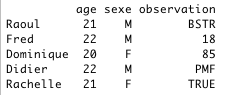
\includegraphics[scale=0.5]{dataframes}
\end{flushleft}
\item Créer des tableaux de données : \textit{data.frame()}, les arguments : 
\begin{itemize}
\item autant de vecteurs que de colonnes (le remplissage des dataframes se fait en colonne).
\item (optionnel) \textit{row.names} pour spécifier le nom des lignes
\item (optionnel) \textit{stringsAsFactors = TRUE/FASLE}, compostement à utiliser avec les vecteurs contenant des chaînes de caractères
\begin{itemize}
\item \textit{TRUE : } convertion auto de vecteurs en facteurs
\item \textit{FALSE : } ces vecteurs restent des vecteurs
\end{itemize}
\end{itemize}
\item Autre déclaration : 
\newline \textit{data.fram(taille=vect1, poids=vect2, ..., row.names = c("A","B",...))}
\item Comme les éléments d'une même colonne peuvent avoir des types différents il faudra parfois utiliser des facteurs et non des vecteurs pour spécifier le contenu d'une colonne.
\item Accéder aux éléments des dataframe : mêmes méthodes que les matrices
\item Méthodes spécifiques aux dataframes : 
\begin{itemize}
\item Extraire une colonne : \textit{dataframe\$colonne}
\end{itemize}
\end{itemize}

\subsection{Les listes}
\begin{itemize}
\item Une liste est un ensemble d'éléments ordonnés les uns à la suite des autres dans une même structure indexée. Ces éléments peuvent être de types différents.
\item Leur utilité est de regrouper dans un même objet une série d'autres objets appartenant par exemple à une même expérience ou observation. Il est aussi possible de traiter tous les éléments d'une même liste en une seule fois grâce à des fonctions adaptées.
\item Les lignes ne sont pas nécessairement de la même longueur
\item Traiter des jeux de données différents (nombre, type, etc) sans avoir à répéter la même procédure à chaque fois.
\item Représentation d'une liste sous R (\textit{ex : }Présence de vecteurs de type numérique qui sont associés à un index dont le nom commence par un dollar (\$))
\begin{flushleft}
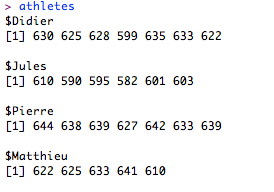
\includegraphics[scale=0.5]{liste}
\end{flushleft}
\item Créer une liste : \textit{list(nom1=vect1, nom2=vect2,...)}
\item Longueur de la liste (nombre de lignes) : \textit{length(liste)}
\item Noms de la liste (nom des lignes) : \textit{names(liste)}
\item Indexation particulière puisque présence de double crochet : \textit{liste[[index/nom]]}
\newline Les index peuvent être les indice des éléments ou les noms associés aux éléments. 
\item Accéder à une ligne : \textit{liste\$nomLigne}
\item Appliquer une même fonction aux différents éléments de la liste : 
\newline \textit{lapply(x, FUN, ...)} (renvoie une liste)
\begin{itemize}
\item \textit{x : } nom de la liste à traiter
\item \textit{FUN : } le nom de la fonction à appliquer à tous les éléments de \textit{x}
\item \textit{... : } arguements optionnels seront les arguments additionnels que peut prendre \textit{FUN}, par exemple \textit{na.rm}
\end{itemize}
\item Même utilisation que \textit{lapply()} mais qui renvoie les résultats sous la forme d'objet plus utilisable comme vecteurs, matrices ou dataframes : \textit{sapply()}\\
\item Grâce à \textit{sapply()} il est alors possible d'utiliser des fonctions telles que \textit{summary} : \textit{sapply(liste, summary)}
\newline (possible avec \textit{lapply()} mais les résultats ne sont pas bien visibles
\end{itemize}

\end{document}








